\usetikzlibrary{shapes.misc}

% From http://tex.stackexchange.com/questions/123760/draw-crosses-in-tikz
\tikzset{cross/.style={cross out, draw=black, fill=none, minimum size=2*(#1-\pgflinewidth), inner sep=0pt, outer sep=0pt}, cross/.default={2pt}}

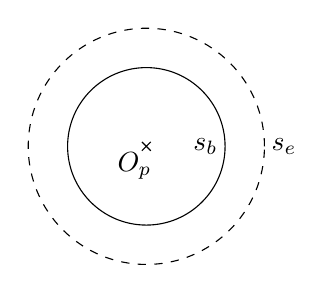
\begin{tikzpicture}

\draw  (0,0) node (v1) {} ellipse (1 and 1);
\draw [dashed] (v1) ellipse (1.5 and 1.5);
\node at (0.75,0) {$s_b$};
\node at (1.75,0) {$s_e$};
\node at (-0.15,-0.25) {$O_p$};
\draw (0,0) node[cross] {};
\end{tikzpicture}